\paragraph{MP001 - Schedule Variance}\mbox{}\\[0,3cm]

    % 
    % VALUTARE SE METTERE ANCHE MANUALE SVILUPATORE E ALLEGATO TECNICO CHE NON ERANO STATI PREVENTIVATI
    % SE LE METTI VALUTA LA POSSIBILITA DI AGGIUNGERE ULTERIORI RITARDI PER ALTRE ATTIVITA CHE COSI PUOI GIUSTIFICARLE
    % 
    \begin{table}[H]
        \centering
        \begin{tabular}{cccc}
            \rowcolor{greySWEight}
            \textcolor{white}{\textbf{Attività}} & 
            \textcolor{white}{\textbf{Abbreviazione}} &
            \textcolor{white}{\textbf{Valore Indice}}&
            \textcolor{white}{\textbf{Riscontro}}\\
            \textbf{Incremento Glossario} & GLO & -1 & \textcolor{ForestGreen}{Ottimale} \\
            \textbf{Incremento Piano di Qualifica} & PDQ & 0 & \textcolor{ForestGreen}{Ottimale} \\
            \textbf{Incremento Piano di Progetto} & PDP & -1 & \textcolor{ForestGreen}{Ottimale} \\
            \textbf{Incremento Norme di Progetto} & NDP & 0 & \textcolor{ForestGreen}{Ottimale} \\
            \textbf{Codifica} & CO & 1 & \textcolor{YellowOrange}{Accettabile} \\
            \textbf{Manuale utente} & MU & 0 & \textcolor{ForestGreen}{Ottimale} \\
            \textbf{Manuale Sviluppatore} & MS & 0 & \textcolor{ForestGreen}{Ottimale} \\

        \end{tabular}
        \caption{Schedule Variance alla revisione di Approvazione}
    \end{table}
    \begin{figure}[H]
        \centering
        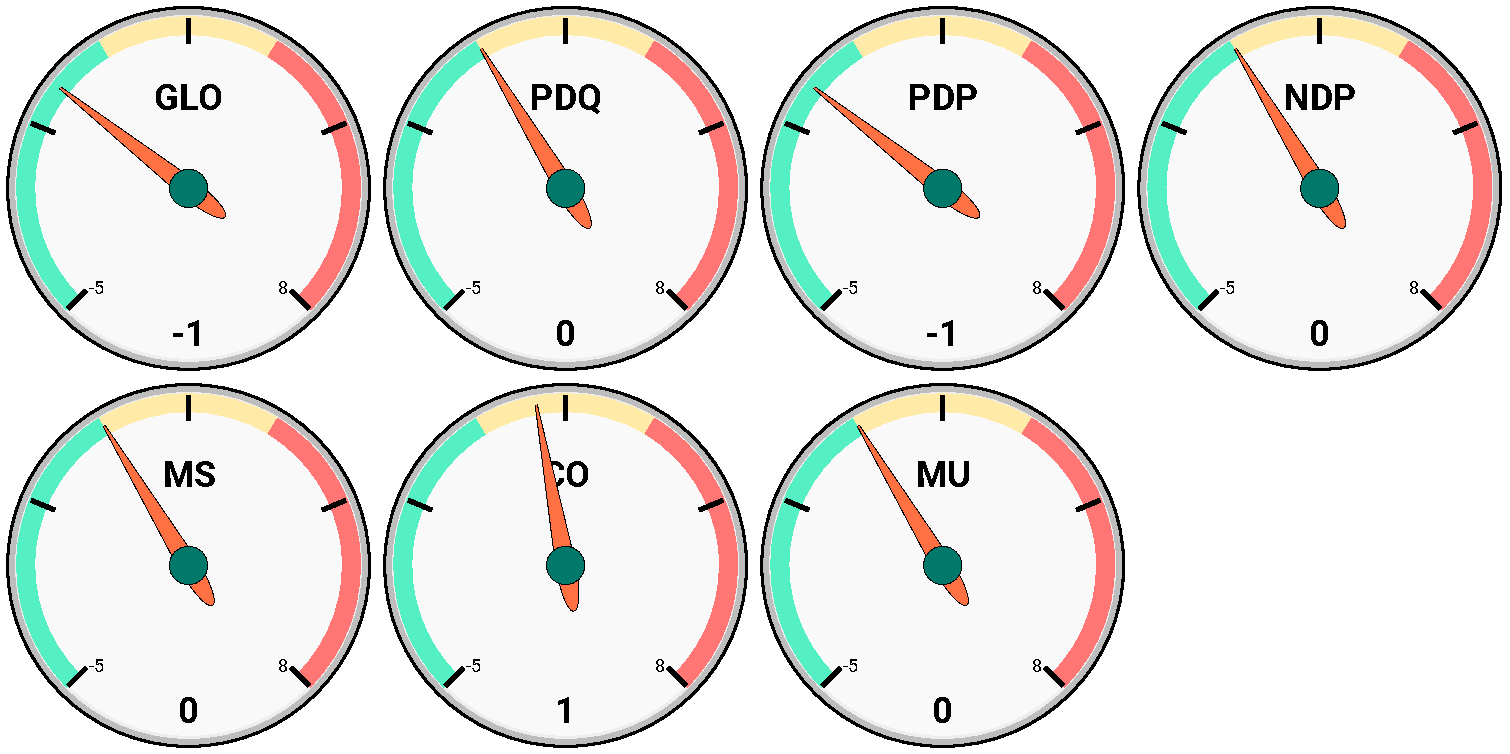
\includegraphics[width=0.9\linewidth]{sez/App_Esito/Approvazione/graph/scheduleVarianceRA.pdf}
        \caption{Schedule variance alla revisione di Approvazione}
    \end{figure}
\paragraph{MP002 - Budget Variance}\mbox{}\\[0,3cm]
    \begin{table}[H]
        \centering
        \begin{tabular}{cccc}
            \rowcolor{greySWEight}
            \textcolor{white}{\textbf{Codice}} &
            \textcolor{white}{\textbf{Valore Indice}}&
            \textcolor{white}{\textbf{Valore in €}}&
            \textcolor{white}{\textbf{Riscontro}}\\
            MP002 & 0.71\% & 21 & \textcolor{ForestGreen}{Ottimale}\\
        \end{tabular}
        \caption{Budget Variance alla revisione di Approvazione}
    \end{table}
    \begin{figure}[H]
        \centering
        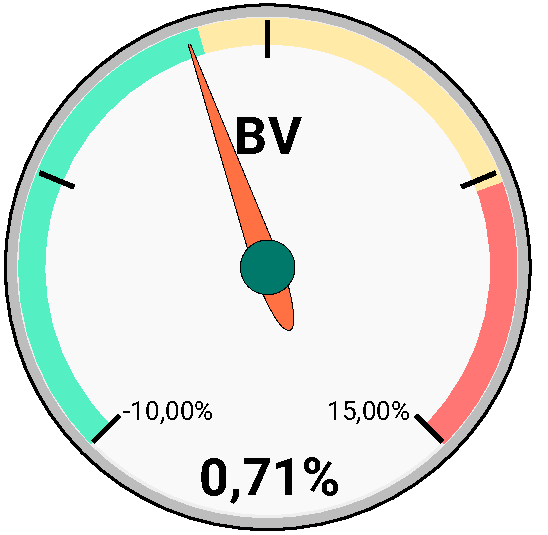
\includegraphics[width=45mm]{sez/App_Esito/Approvazione/graph/budgetVarianceRA.pdf}
        \caption{Budget variance alla revisione di approvazione}
    \end{figure}
    \begin{figure}[H]
        \centering
        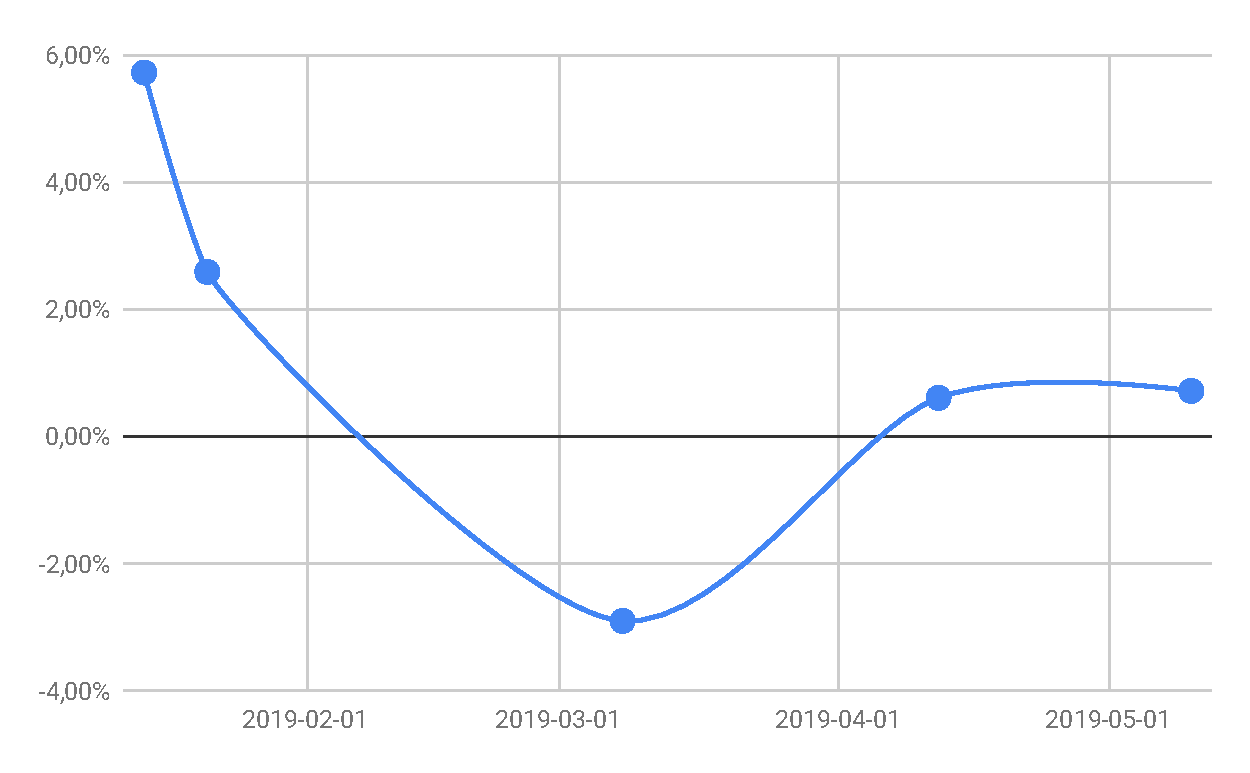
\includegraphics[width=0.7\linewidth]{sez/App_Esito/Approvazione/graph/budgetVarianceRAStorico.pdf}
        \caption{Andamento budget variance fino alla revisione di Approvazione}
    \end{figure}
    \newpage